\section{Neues Projekt anlegen} \label{sec: Neues_Projekt_anlegen}

\subsection{TIA Portal öffnen}
Im PC-Menü \glqq\textbf{Start}\grqq\:nach dem \textbf{TIA Portal} suchen (hier Version: V17) und Software starten.
\begin{figure}[H]
   \centering
   \fbox{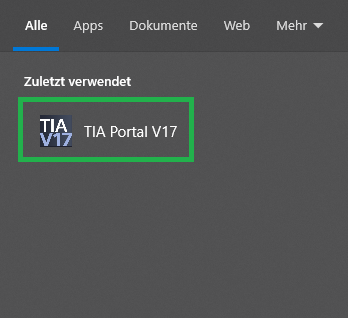
\includegraphics[width=0.4\textwidth]{Bilder/2. Neues Projekt anlegen/(1) TIA Portal V17 oeffnen.png}}
   \caption[TIA Portal öffnen]{TIA Portal öffnen}
   \label{fig:Bild2.1}
\end{figure}

\subsection{Projekt erstellen}
\textbf{Projektname, Pfad} und \textbf{Autor} vergeben und mit \glqq\textbf{Erstellen}\grqq\:bestätigen.
\begin{figure}[H]
   \centering
   \fbox{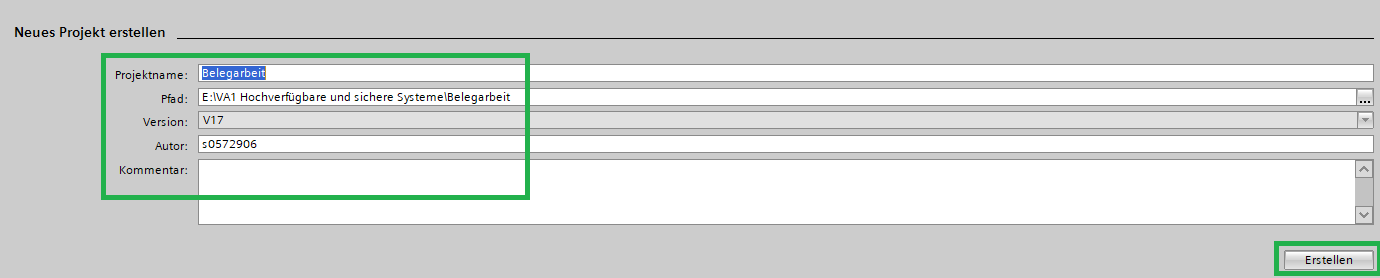
\includegraphics[width=1.0\textwidth]{Bilder/2. Neues Projekt anlegen/(2) Neues Projekt erstellen.png}}
   \caption[Neues Projekt erstellen]{Neues Projekt erstellen}
   \label{fig:Bild2.2}
\end{figure}

\clearpage

\subsection{Projektansicht öffnen}
Die Projektansicht über \glqq\textbf{Projektansicht öffnen}\grqq\:aufrufen und weitere Einstellungen vornehmen.
\begin{figure}[H]
   \centering
   \fbox{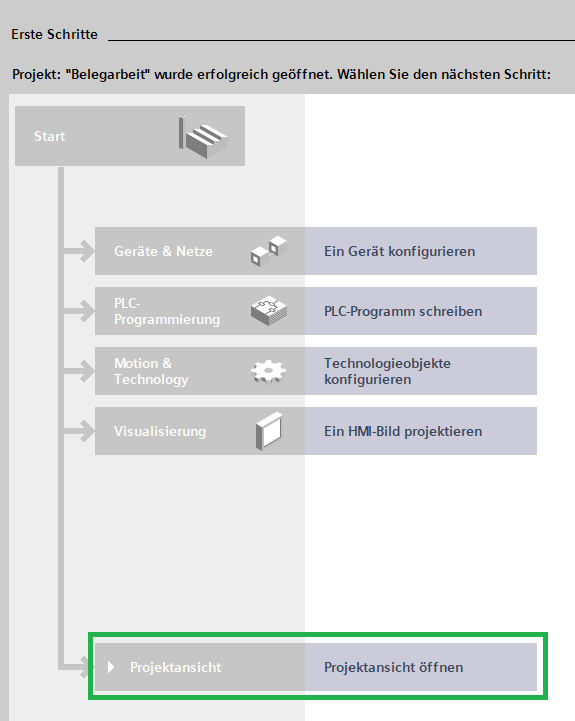
\includegraphics[width=0.6\textwidth]{Bilder/2. Neues Projekt anlegen/(3) Projektansicht oeffnen.png}}
   \caption[Projektansicht öffnen]{Projektansicht öffnen}
   \label{fig:Bild2.3}
\end{figure}